\documentclass[12pt]{article}

\usepackage[margin=1.125in]{geometry}
\usepackage[utf8]{inputenc}
\usepackage[english]{babel}
\usepackage[doublespacing]{setspace}
\usepackage[T1]{fontenc}
\usepackage{lmodern} % To switch to Latin Modern
\rmfamily % To load Latin Modern Roman and enable the following NFSS declarations.
% Declare that Latin Modern Roman (lmr) should take
% its bold (b) and bold extended (bx) weight, and small capital (sc) shape, 
% from the corresponding Computer Modern Roman (cmr) font, for the T1 font encoding.
\DeclareFontShape{T1}{lmr}{b}{sc}{<->ssub*cmr/bx/sc}{}
\DeclareFontShape{T1}{lmr}{bx}{sc}{<->ssub*cmr/bx/sc}{}

% \usepackage{lmodern}
\usepackage{amssymb,amsmath}
\usepackage{longtable}
\usepackage{booktabs}
\usepackage{appendix}
\usepackage{cprotect}
\usepackage{comment}
\usepackage{pdfpages}
\usepackage{subcaption}

\graphicspath{ {assets/} }

\usepackage[autostyle]{csquotes}
\MakeOuterQuote{"}

\usepackage{listings}
\lstset{
  columns=fullflexible,
  frame=single,
  breaklines=true,
  postbreak=\mbox{\textcolor{red}{$\hookrightarrow$}\space},
}
 
\setcounter{tocdepth}{1}

\usepackage[margin=.5cm]{caption}
\captionsetup{font=doublespacing}% Double-spaced float captions
% \captionsetup{margin=3cm} inside a figure
% to change only that figure
 
 \usepackage[
 backend=biber,
 citestyle=ieee
 ]{biblatex}
\addbibresource{main.bib}
\usepackage{chngpage}

\usepackage{etoolbox}
\AtBeginEnvironment{equation}{\leavevmode\singlespace}
\AfterEndEnvironment{equation}{\endsinglespace\vskip0.5\baselineskip\noindent\ignorespaces}


\makeatletter
\DeclareRobustCommand{\KaTeX}{K%
  {%
    \setbox0\hbox{T}%
    \setbox\@tempboxa\hbox{$\m@th$%
      \csname S@\f@size\endcsname
      \fontsize\sf@size\z@
      \math@fontsfalse\selectfont
      A}%
    \@tempdima\ht0
    \advance\@tempdima-\ht\@tempboxa
    \@tempdima\strip@pt\fontdimen1\font\@tempdima
    \advance\@tempdima-.25em
    \kern\@tempdima
    \vbox to\ht0{\box\@tempboxa
      \vss}%
  }%
  \kern-.15em
  \TeX}

\makeatother

\setlength{\parindent}{0em}
\setlength{\parskip}{.5em}
\newcommand{\TeXNet}{Hunter \TeX Net}
\newcommand{\BLEU}{\textsc{Bleu}}

\title{\TeXNet{} \textbar{} CSCI 350 Final Project}
\author{Alex Taradachuk \and Ralph ``Blake'' Vent\'{e}}
\date{March 2020}

\begin{document}

\maketitle

\begin{abstract}
  The OpenAI request for research spawned investigation into visual neural
  models for translating mathematical expressions into markup code. Since the
  debut, progress has been largely incremental. Singh 2018, Wang 2019, and
  Bender 2019 all attribute properties of their respect models to the biases in
  the corpus and its pre-processing. We present a new dataset of 170,000
  rendered examples and 500,000 normalized formulas along with a pipeline for
  harvesting examples from source files hoping to minimize these biases. We
  train a Convolutional Neural Network with Long-Short Term Memory Cells and an
  attention mechanism to a testing accuracy of 0.87 bigram \BLEU{} score.
\end{abstract}

\begin{singlespace}
\tableofcontents
\end{singlespace}

\section{Previous Work}

\subsection{Debut}

The prospect of accurately transcribing mathematical expression into a markup
representation is enticing because it opens the doors for bringing new life to
old mathematical texts or those for which the source code is unavailable.

\citetitle{deng2016you} by~\citeauthor{deng2016you}
documents strategies for machine translation of mathematical notation using an
attention-based encoder-decoder neural model. Notably, the researchers were
interested in the influence of markup alone on the efficacy of a model ---
without providing explicit information about underlying grammars
\parencite[1]{deng2016you}. The previous state of the art required exhaustively
documenting the grammar to allow a conventional character recognition model to
translate the expression.

Introduced in 2016 by~\citeauthor{deng2016you}, the \texttt{im2latex100k} dataset has
facilitated research by reducing the overhead of heavy pre-processing. Using
this dataset, other solutions to \textsc{im2latex} have seen substantial
progress. Recently, it has come under scrutiny as a possible \textit{bottleneck} for
progress. We discuss this in greater detail in Section~\ref{datainnov}.

\cprotect
\subsection{\textsc{im2latex} Problem Specification}

Before delving into how architectures were designed to solve the problem, let us
first define it. Formally, this problem is a sequence-to-sequence image
captioning task. A neural model learns an abstract encoding and its respective
decoding into the original sequence \parencite[1]{deng2016you}. At inference
time, when presented a single image, the trained model predicts one token at a
time, aiming to reconstruct the original sequence. All the while, the model
receives as input the output of previous steps. This is accomplished using
Long-Short Term Memory, which we outline in \ref{netarch}.

\subsection{Architectural Designs}
\label{netarch}

Since its inception, solutions to \textsc{im2latex} have used neural models. In
fact, OpenAI's Request for Research recommended the use of a neural model and
even specified the sequence-to-sequence attention machanism that makes these
models suitable for the problem, but there have been a wide variety in the
particular architectures of the neural models.

The authors \citeauthor{deng2016you}, \citeauthor{genthial2016image},
\citeauthor{wang2019translating}, and \citeauthor{bender2019learning} all
iteratively build on the models before them and experience iteratively better
results.

We proceed with Singh's model for our architecture which notably does away with
max-pooling layers at no cost to performance. Details about its convolutional
encoder, attention model, and decoder are all found starting with
\cite[3]{singh2018teaching}. Our only change to the model was to expand the
number of output units from 50 to 64 to suit our dataset's more diverse
vocabulary.

\section{Corpus Harvesting}


\subsection{Challenges}

We harvested examples from Cornell's arXiv journal. As the arXiv strictly
forbids scraping, we discovered that a generous archivist properly obtained
copies (paying for transfer from Amazon s3 buckets) and uploaded them to
\url{archive.org}. We wrote a script to extract the source code files, and
notably, we use the \texttt{pandoc} document parser.

On this note, \LaTeX{} and its subset, \TeX{} pose an unique set of challenges
compared to other steps of the pre-processing pipeline. \LaTeX{} is a
Turing-Complete language, equivalent in power to general purpose programming
languages. From the theoretical standpoint, it may contain loops and recursion,
classifying it as a recursively enumerable language. As such, no \LaTeX{} parser
is guaranteed to terminate, and regular expressions alone lack the expressive
power to extract all cases of a particular pattern. Practically, we mostly
needed to contend with macro expansion whereby commands used as contractions
needed expanding into their definition. This means that the original scripts of
\cite{deng2016you} required substantial changes before being suitable for our
purposes.

\subsection{Innovations}
\label{datainnov}

To start, we follow closely in the footsteps of~\citeauthor{singh2018teaching}. After
preprocessing steps on \texttt{im2latex100k}, Singh arrived upon a dataset of
93,784 compiling examples, which he regarded as ``too small for good
generalization.'' As such, he mined additional examples from the KDD Cup 2003
dataset, resulting in about additional 50,000 examples
\parencite[8]{singh2018teaching}.  % also
                                % mention that the others have issues w data[]

Practically, \texttt{pandoc} handled the files from the corpus gracefully, but
due to unlinked files and mismatched encodings, we set \texttt{timeout 5} to
terminate the program after 5 seconds of stalling. \texttt{pandoc} also
facilitates extracting expressions. Without it, we were presented with the
challenging prospect of filtering out text not containing mathematical
expressions, but \texttt{pandoc} generates an abstract syntax tree and encases
the mathematical expressions in the more ``specific'' expression
\verb|\((.*?)\)| compared to the expression \texttt{\$(.*?)\$} which resulted in
false matches that contained only text. One such false match that was eliminated
is provided in Figure~\ref{falsematch}. As a fall-back, we rely on Singh's script to test
for the presence of at least one \LaTeX{} command (from the command vocabulary,
$\Sigma$) before writing out the final formula code. This has the added benefit
of removing examples that are strictly numbers and those that are otherwise
linear strings of alphanumeric characters.

Most importantly, \texttt{pandoc} expands all the macros in the source
documents. Without this step, papers in the dataset that relied heavily on
macros to shorten the length of the written expressions contributed very few
formulas to the resulting collection because they caused definition-not-found
errors and were eliminatedin later steps. In~\cite{deng2016you} the processed
formulas were discarded implicitly because they caused such errors, but with the
macros expanding, documents containing macros reclaimed their representation in
the final set, eliminating one possible source of bias in the dataset.

The pipeline allows us to diverge from using the KDD-Cup 2003 as a data source.
To us, this means the data is not representative of math as a whole. From this
standpoint our data is free of such a bias.

%\begin{figure}[!h]
\begin{figure}[tbp]
\begin{adjustwidth}{-1in}{-1in}% adjust the L and R margins by 1 inch
		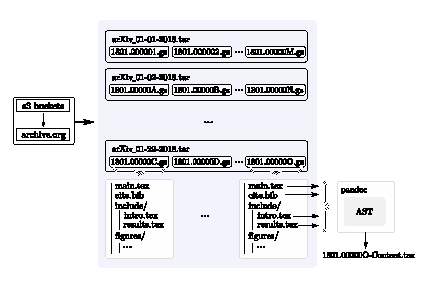
\includegraphics[scale=2.0]{harvest.pdf}
    \centering
\end{adjustwidth}
    \cprotect\caption{Examples flow from the Internet Archive and are stored on
    our disks, where we extract the \texttt{tar} files first by day, then by
    submission, into the document folders. Then \texttt{pandoc} pulls in all of
    the dependencies of this particular document and writes out one stand-alone
    document with macros expanded. Then we match the regular expression
    \verb|\((.*?)\)| that \texttt{pandoc} uses to wrap mathematical expressions.
    As a general tool \texttt{pandoc} can convert between other markup language
    in the same way, making it useful for standardizing data from disparate
    sources. Special thanks to Brian Newbold \url{http://bnewbold.net/}, an
    internet archivist, working at the Internet Archive who provided the raw
    form of the data we pre-processed.}\label{datapipeline}
\end{figure}

From~\citeauthor{deng2016you}, we also reiterate that several \LaTeX{} input sequences
map to the same output image, so we use the same normalization with Khan
Academy's \KaTeX{} as they did in their scripts. Like \texttt{pandoc}, \KaTeX{}
parses the input sequences into an abstract syntax tree and rebuilds the
expressions without disrupting
semantics. 

\citeauthor[5]{bender2019learning} note that their \textsc{im2latex} model struggled
very short sequences, and performed better on those that were slightly longer.
They attribute this to an imbalance in the dataset: very short formulas are
underepresented. In fact, this may be traced back to the scripts written by
\cite{deng2016you}, which discarded examples shorter than 40 bytes in length. We
halved the minimum length of an example.

\subsection{Product}

In all, we mined 1 month of \texttt{tar} files, extracted 15,200 \texttt{tex}
files, expanded macros 7,200 unique files and generated data 500,000
syntactically valid examples. We decided to randomly subsample about 40\% of
that as our final candidate set. After deduplicating, we were left with 170,00
original examples. Our formula files can be found
at~\url{https://github.com/rvente/TeXNet.ai/Dataset .} A graphical view of our
data pipeline can be seen in Figure~\ref{datapipeline}.

\section{Network Architecture}

Our network is based on \citeauthor{singh2018teaching}'s research. The general
architecture has several essential features that we enumerate with brief
explanations then proceed with detailed remarks on their relevance to our
architecture.

\begin{description}
  \item[Convolutional Neural Network (CNN)] Layers in our neural model learn
  convolutions on pixel space that extracts meaningful information into a
  compressed internal embedding, that is, a vector which has a dense encoding of
  the contents of the input image.
  \item[Recurrent Neural Network (RNN)] This allows for reasoning over time
  because information from prior time-steps can factor into current time steps.
  It accomplishes this by incorporating as input the output of previous layers.
  \item[Long-Short Term Memory (LSTM)] Looseley speaking, the LSTM cells in the
  neural network "learn what to forget and when to forget it." This aspect of
  the architecture allows a particular subset of the previous layer's output to
  be factored in dynamically based on what the LSTM cells have learned is
  important.
  \item[Attention machanism] Attention mechanisms allow for the network to mask
  way, or "ignore" portions of the input image. The network can now use
  information about past predictions to "keep track of where it's looking," allowing
  for focused steps in the prediction process.
\end{description}

\subsection{Convolutional Neural Network}

A deep CNN is used to encode preprocessed input images into a \textit{visual
feature grid} composed of \textit{visual feature vectors}. These feature vectors
are then pooled to get \textit{pooled feature vectors}. Each pooled feature
vector acts as a rectangular window into the pooled images which partitions the
image into spatially localized regional encodings \parencite{singh2018teaching}.
Encoding features in this piecewise manner allows for a decoder artchitecture
that places focus on select regions at a certain time-step while de-emphasizing
the rest. Additionally, we are able to construct different encoded features by
specifying receptive field sizes during pooling. After pooling, the resulting
sequence of pooled feature encodings are passed to the decoder.

By contrast, Singh's \texttt{NOPOOL} model removed the max pooling layers which
improved the rate of convergence and lowered training times, yet the performance
difference without max pooling to the 

\subsection{Recurrent Neural Networks}

At time $t$, the an RNN's layer $n$ takes as input the output of layer $n$ at
time $t-1$. To train such a network using backpropagation, it is "unrolled" so
as to emulate a feed-forward network, allowing the updates to propagate. The
issue with an RNN alone is that memory of previous inputs quickly decay when
moving from time-step to time-step. 

\subsection{Long-Short Term Memory Configuration}

To solve these issues, researchers use need a network to selectively add and
remove inputs into the current state \parencite{zhang2019dive}. Dating back to
1997, this LSTM architecture solves this using gates to control the flow of data
during training and inference \parencite{zhang2019dive}. It takes 3 inputs,
$c_{t-1}$ memory at time $t-1$ (context), the previous hidden state's output
$h_{t-1}$ and of course the new sequence at the current time-step $x_t$.
\citeauthor[12]{singh2018teaching} documents the specifics of the model we use
in great detail.

\section{Training and Evaluation}

\begin{figure}[!h]
  \begin{subfigure}{0.5\textwidth}
		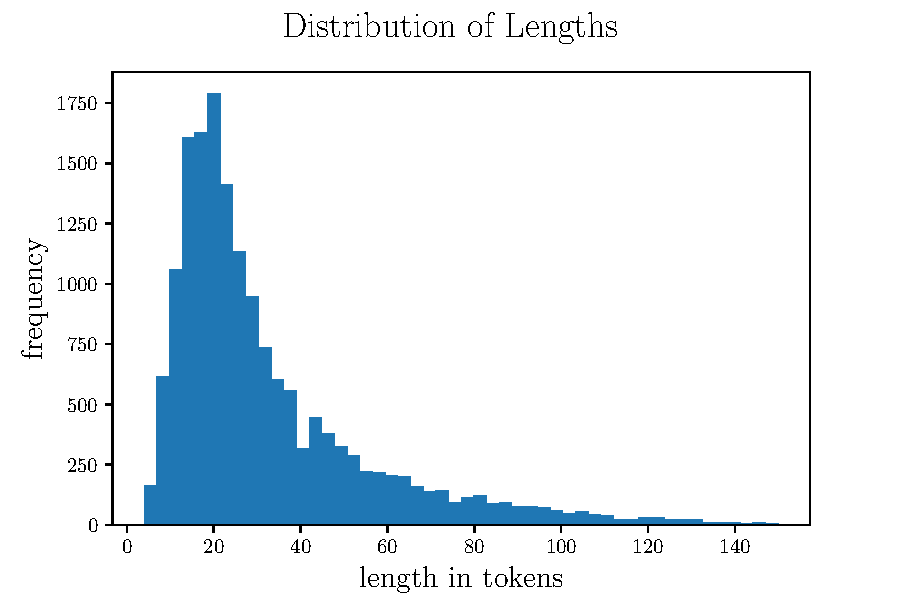
\includegraphics[scale=.425]{histogram.pdf}
		\centering
		\caption{}
	\end{subfigure}
	\begin{subfigure}{0.5\textwidth}
		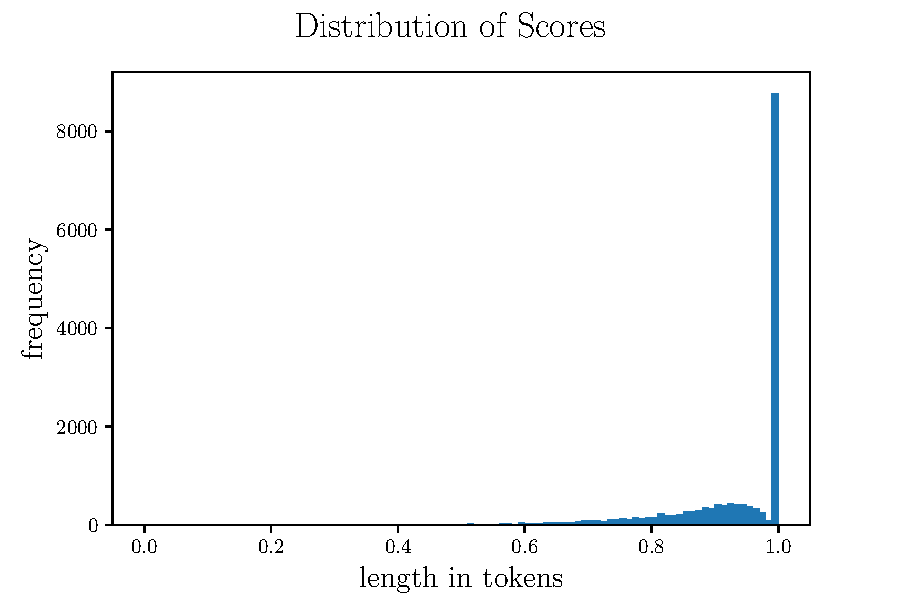
\includegraphics[scale=.425]{scorehistogram.pdf}
		\centering
		\caption{}
	\end{subfigure}
  \begin{subfigure}{1.0\textwidth}
		\centering
		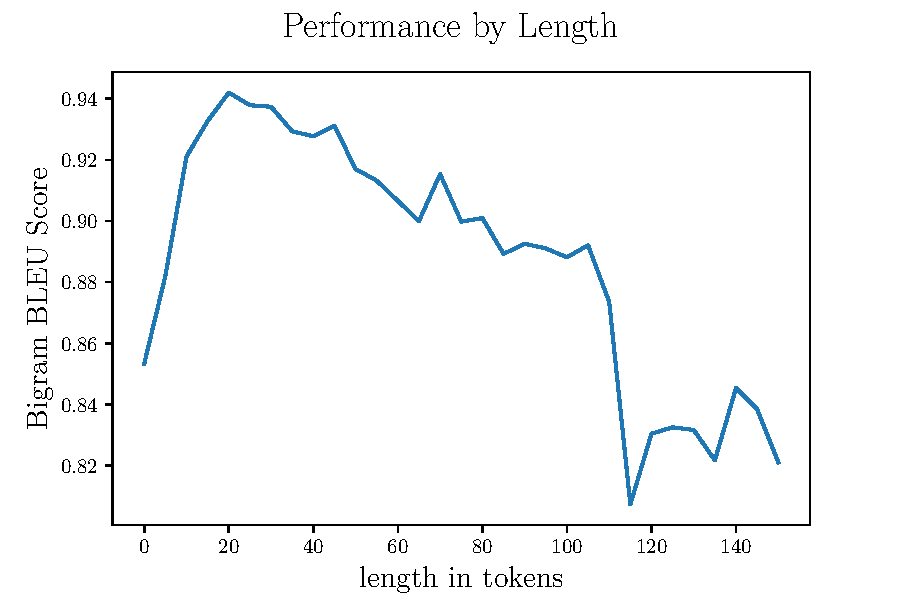
\includegraphics[scale=.425]{scorebylen.pdf}
		\caption{}
	\end{subfigure}
  \caption[Model]{This assessment is on the validation set $N=16,520$. (a)
  Plotted with 50 bins. The mean length is with a mean of  32.56 and standard
  deviation of 23.82. (b) Plotted with 100 bins. \BLEU{} Scores are strongly
  concentrated on 1.0, with $\mu = 92.5$ and $\sigma = 23.81$. It seems that the
  discontinuous indentation before 1.0 is an artifact of how \BLEU{} score
  penalizes non-perfect matches. There, a single incorrect token causes bin. (c)
  As expected, performance is inversely proportional to length, however on the
  longest tokens, the model still perfomed at a respectable .82 \BLEU{} score.
  The model seems to be generalizing well -- it doesn't need to see every token
  in every configuration to make an accurate prediction. The steep drop-off
  after 100 tokens is caused in part by there being fewer examples contributing
  to the average on that bin, so a few uncharacteristically bad predictions have
  a large influence. } 
\end{figure}

We trained the neural network on a Virtual Machine (VM) with an NVIDIA Tesla
V100. Later, that platform became unavailable, so we migrated training to a VM
with an NVIDIA Tesla P1 instead. Unfortunately, this change means we cannot make
conclusions about the seconds to convergence between datasets of different size.

For evaluation, we use Bilingual Evaluation Understudy (\BLEU{}), the emerging
standard among neural network solutions to the \textsc{im2latex} problem. \BLEU{}
is an automated metric for assessing machine translation accuracy
\cite[1]{papineni2002bleu}. It is computed by comparing a target translation
(ground truth) to the predicted sequence.

We report 3 metrics: first we compute global \BLEU{} score across all examples and
then again with 2 splits. The first split evaluates performance by length in
tokens of the target sequence and the next split evaluates performance based on
the contents of the expression.

We selected 3 "categories," chosen based on the qualities of the expression. For
Group A, we select expressions containing matrices, arrays, and piece-wise
functions (cases). For Group B, we select those containing fractions. We leave
the rest of the data in Group C. We note that the sets not disjoint.
\begin{figure}[h]
	\begin{subfigure}{0.5\textwidth}
    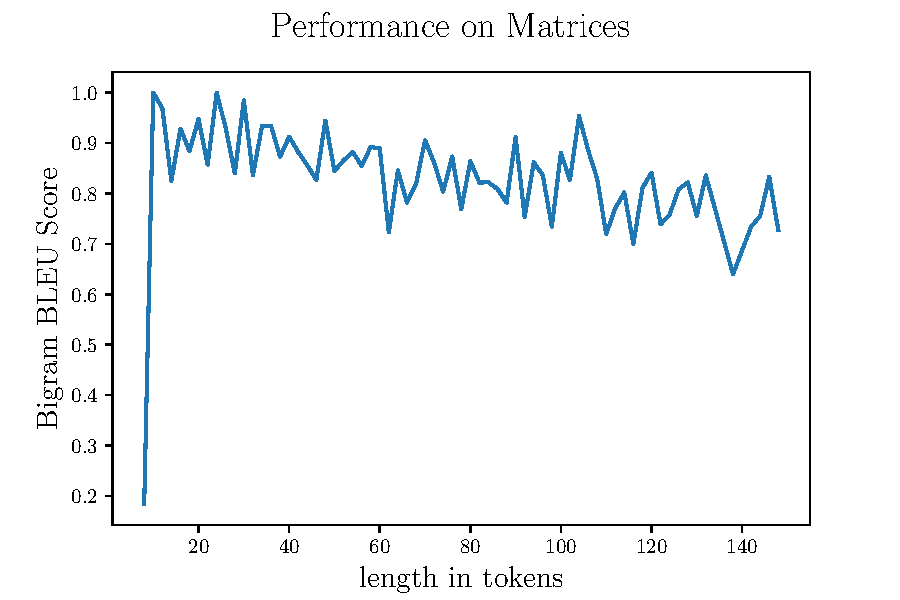
\includegraphics[scale=.425]{scorebylenstacked.pdf}
    \centering
		\caption{}
	\end{subfigure}
  \begin{subfigure}{0.5\textwidth}
    \centering
		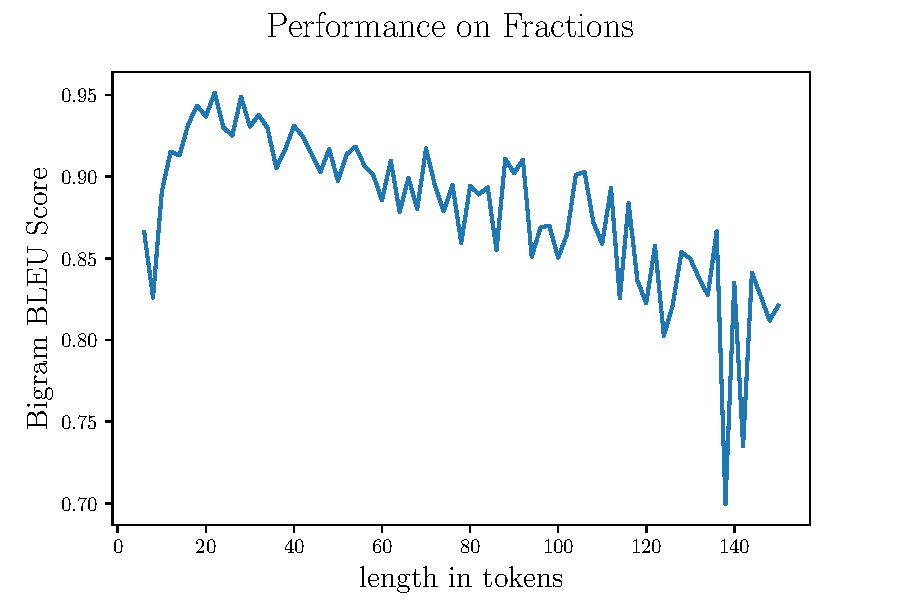
\includegraphics[scale=.425]{scorebyfrac.pdf}
		\caption{}
  \end{subfigure}
  \caption[Model]{(a) We generalize cases (peicewise functions), arrays,
  matrices, column vectors here and evaluate performance on that set finding
  $\mu = 0.85, \sigma=0.14$. Unsurprisingly, matrices were more challenging for
  the model than general math, but matrices are underepresented at $N=291$ (b)
  We match \texttt{frac} and \texttt{over} for fractions finding $\mu = 0.91$
  and $\sigma =0.11$ Samples $N = 2897$.}
\end{figure}

From \citeauthor{papineni2002bleu}, \BLEU{} score has a penalty for translations
that are too long and those which are too short. The former case is handled
implicitly, and the latter requires an explicit brevity penalty, $\text{BP}$
computed as
\begin{equation}
 \text{BP} = \begin{cases}1 &\text{ if } c>r \\
  e^{1-r/c} &\text{ otherwise }\end{cases}.
\end{equation}
with $r$ as the length of of the ground-truth sentence and $c$ as the length of
the candidate sentence. Then, we have 
\begin{equation}
  \text{\BLEU} = \text{BP} \exp\left( \sum_{i=1}^n w_i \log p_i \right),
\end{equation}
where $p_n$ is geometric mean of $n$-gram precisions from 1 to $N$ and $w_n$ is
a parameter weight, such that $\sum_i w_i = 1$. \citeauthor{papineni2002bleu}
used $w_n = 1/N$. \citeauthor{papineni2002bleu} show that \BLEU{} score is
predictive of human judgements, resulting in its widespread use in translation
tasks.

We use the same reformulation of this metric as \parencite{singh2018teaching}
and \parencite{deng2016you}, the bigram \BLEU{} (\BLEU{}2) score computed with
$w_1=w_2=.5$ and $w_i = 0$ for $i>2$. Also like Singh, the scores we report
actually compare non-normalized target sequences to the normalized predicted
sequences, resulting in a pessimistic predictive score because the network was
not trained on this sequence. Despite this, the \BLEU{}2 scores are quite
satisfactory.

% This might indicate that the majority of input sequences in our
% \texttt{im2latex170k} corpus were fairly close to being normalized. We can
% test this by comparing the normalized corpus to the non-normalized one.
\begin{figure}[!ht]
  
\begin{longtable}[]{@{}ll@{}}
\toprule
Researchers & BLEU Score (\%) \tabularnewline
\midrule
\endhead
Deng et al 2017 & 87.73 \tabularnewline
Genthial 2017 & 88.00 \tabularnewline
Wang, Sun \& Wang 2018 & 88.25 \tabularnewline
Singh 2018 & 89.00 \tabularnewline
\textsc{texnet} & 88.48 \tabularnewline
Wang \& Liu 2019 & 90.28 \tabularnewline
\bottomrule
\end{longtable}\caption{Performance alongside other solutions to \textsc{im2latex}}
\end{figure}


\subsection{Limitations and Future work}

Through the testing of our current model, we have observed notable performance
decrease with increasing sequence length. This is most likely due to the low
proportion of training data sequences over 140 symbols however it could also be
a result of a loss in resolution as sequence length increases. A next step
forward could include partitioning the data if sequence length is long enough.
Additionally, the preprocessing scripts utilized by Singh
\parencite{singh2018teaching} leave a white outline around the images generated
from \LaTeX\ which the network is hardwired to expect. As a result, in order for
the model to work on pulled examples from the internet, we had to preprocess the
images in the following manner using \texttt{imagemagick}'s \texttt{convert}
utility:
\begin{enumerate}
  \item Crop formula to reduce outside padding and resize image to fit under the
  128 pixel token height limit (if needed)
  \vspace{1em}
  \begin{lstlisting}[basicstyle=\ttfamily]
    convert <input-img> -resize x90 <output-img>
  \end{lstlisting}
  \item Make the white background transparent with a fuzz of 5\% to account for
  the feather expected by the model
  \vspace{1em}
  \begin{lstlisting}[basicstyle=\ttfamily]
    convert <white-img> -fuzz 5\% -transparent white <preproc-img>
  \end{lstlisting} 
\end{enumerate}

The use of our own data, scraped from real world examples, lended our model to
be more accurate when it came to inferencing specific downloaded images.
However, there was a disparity in training time between Singh's model and ours,
despite having similar BLEU scores (88.7), which could've impacted results. For now,
the current model is effective only on \LaTeX{} default typeface of Computer
Modern, but preprocessing steps can be applied to make the model more invariant
to typefont of data. As a proof of concept however, building im2latex models
with deeper layers and increasing data size is promising given our results and
the general trend NPL models are currently taking.

In the future, there might be a chance to explore the use of GRU (gated
recurrent unit) cells instead of LSTM cells. According to
\citeauthor{zhang2019dive}, GRU cells are much less computationally insensive
and may make deeper models more practical. Paired with the densenet approach in
\cite{wang2019translating}, GRU's might allow for such an architecture to reap
the benefits of deepening.

Our final piece of future work is a cross comparison between our datasets: we
want to see hour our model fares against \texttt{im2latex100k} and
\texttt{im2latex140k}. Given more time, we would compare performance on all
available models and all available data. 

\newpage
\begin{appendix}
  \section{Qualitative Analysis}
  \subsection{Reducing Plain Text Matches}

\begin{figure}[!h]
  \qquad \textbf{The source code}
  \begin{lstlisting}[escapechar=!, basicstyle=\footnotesize\ttfamily, numbers=left, firstnumber=1132]
    The net flow vector $(1,1,0,\hdots,0)$ has previously been considered for the complete graph by Corteel, Kim, and M\'esz\'aros \cite{CKM}.  They used the Lidskii formula~\eqref{eq:lidskiivol} and constant term identities to derive the following product formula for the volume of $\mathcal{F}_{K_{n+1}}(1,1,0,\ldot     s,0)$.
    It would be of interest to rederive this result using the refined Kostant constants.
   \begin{theorem}[{\cite[Theorem 1.1]{CKM}}] \label{thm:volkn11}
   Let $n\geq 1$. For the complete graph $K_{n+1}$,

  \end{lstlisting}
  \qquad \textbf{matched the regular expression} \verb|$(*.?)$| \textbf{with the string} 
  \begin{lstlisting}[basicstyle=\footnotesize\ttfamily]
  $. It would be of interest to rederive this result using the refined Kostant constants. \begin{theorem}[{\cite[Theorem 1.1]{CKM}}] \label{thm:volkn11} Let $    
  \end{lstlisting}
   \cprotect\caption{From \texttt{arXiv:1801.07684} \citeauthor{benedetti2018combinatorial} }\label{falsematch}
\end{figure}

Figure~\ref{falsematch} is a sample from a particular document whose source code
induced a false match. Math code encased in dollar-signs has been deprecated in
\LaTeX{}, but remains in wide use as an artifact from \TeX{}. It was deprecated
to facilitate parsing: unlike \verb|\(| which indicates that the expression
opens to the right, the dollar-sign gives no such indication. The reason the
previous scripts were matching these plain-text strings was because matching all
strings that start and end in dollar-signs doesn't preclude text from matching.
In this case, the last \verb|$| of the first line matched with the first
\verb|$| of the 4th line. Researchers from \cite[4]{deng2016you} to
\cite{singh2018teaching} have contended with this but our solution doens't
require filtering out long sequences aribitrarily.

  \section{Team Member Roles and Contributions}
    \subsection{Alex}
      \begin{enumerate}
        \item Upgraded Singh's model to Python 3 and got it working with the
        latest version of Tensorflow-GPU v1 (1.15.2 Stable).
        \begin{itemize}
          \item Use of deprecated neural layers slowed porting to Tensorflow v2
          and time constraints led this idea to being scrapped for the time
          being. 
        \end{itemize}
        \item Got the model to begin training on VM, specifically using the dedicated GPU. 
        \item Modified model to be able to take Blake's generated data as input.
        \begin{itemize}
          \item Hard-coded expected vocabulary input had to be changed and number
          of output layers had to be adjusted to the different vocabulary
          size of Blake's data.
          \item Many batch-size assertions had to be removed, which posed the
          risk of data-corruption, but was necessary to get the model running
          and did not pose a problem during training.
        \end{itemize}
        \item Focused on retrieving training metric data and parsing through log files.
        \item Modified outdated Jupyter notebooks into Python 3 scripts to
        perform inference on specified input images in two parts.
        \begin{enumerate}
          \item Prepare the data by generating a vocabulary directory and
          copying over the latest model snapshot to be used in inference.
          \item After the model is run on the data using the specified snapshot,
          a second script outputs the predictions by parsing through the
          logfiles and retrieving \LaTeX{} sequences from a sequences of IDs.
        \end{enumerate}
        \item Experimented with inference given downloaded images from the
        internet and figured out what was necessary to get the model to run
        optimally in this case.
      \end{enumerate}
    \subsection{Blake}
      \begin{enumerate}
        \item Configured the Virtual machines and installed the GPU drivers.
        \item Generated image examples from Cornell's arXiv.
        \begin{enumerate}
          \item Data exploration allowed us to construct our preprocessing pipeline.
          \item Adapted Singh's preprocessing scripts.
        \end{enumerate}
        \item Performed system adminstration, resizing the file system to
        respond to changing needs. 
        \begin{enumerate}
          \item Considering that the dataset was about 700 MB and each snapshot
          of the model weights was 800 MB, we quickly ran out of storage with
          our 32 GB configuration. We required 64 GB in all.
        \end{enumerate}
        \item Rewrote evaluation scripts from scratch to generate graphs of the
        model's performance on different subsets.
      \item Consistently monitored VM during training. We trained 2 models at 25
      and 55 hours for a total training time of 80 hours.
      \end{enumerate}
\begin{figure}[!ht]
\begin{center}
\begin{longtable}{ l l }
\toprule
  Ground Truth & Prediction  \tabularnewline
\midrule
\endhead
$\nu _ { \mathrm { o b s } } \propto r ^ { s - b + 2 g } $&$\nu _ { \mathrm { o b s } } \propto r ^ { s - b + 2 g } $ \\
$| \widehat { f } _ { k } ( x ) | \leq \frac { \epsilon } { 2 } $ & $| \widehat { f } _ { k } ( x ) | \leq \frac { \epsilon } { 2 } $\\
$S ( 8 - 2 4 ) \geq 7 \times 1 0 ^ { - 1 4 } $&$S ( 8 - 2 4 ) \geq 7 \times 1 0 ^ { - 1 4 } $ \\
$\frac { k ^ { 2 } } { a ^ { 2 } H ^ { 2 } } < < 1 $&$\frac { k ^ { 2 } } { a ^ { 2 } H ^ { 2 } } < < 1 $ \\
$4 _ { 1 } ^ { + } \rightarrow 2 _ { 1 } ^ { + } $&$4 _ { 1 } ^ { + } \rightarrow 2 _ { 1 } ^ { + } $ \\
$0 . 8 0 6 5 1 1 \pm 0 . 0 0 0 2 0 6 $&$0 . 8 0 6 5 1 1 \pm 0 . 0 0 0 2 0 6 $ \\
$P ^ { \prime } = P \times _ { H } G L ( W ) $&$P ^ { \prime } = P \times _ { H } G L ( W ) $ \\
$g _ { s } = ( \textbf { g } \cdot \textbf { B } ) / | \textbf { B } | $&$g _ { s } = ( \textbf { g } \cdot \textbf { B } ) / | \textbf { B } | $ \\
$\{ 5 , 5 , 5 , 5 \} \to \{ 5 , 5 , 5 , 5 \} $&$\{ 5 , 5 , 5 , 5 \} \to \{ 5 , 5 , 5 , 5 \} $ \\
$\theta _ { 1 } = \theta _ { 2 } = \lambda _ { l } $&$\theta _ { 1 } = \theta _ { 2 } = \lambda _ { l } $ \\
$h _ { r m s } = 6 \times 1 0 ^ { - 1 0 } m $&$h _ { r m s } = 6 \times 1 0 ^ { - 1 0 } m $ \\
\bottomrule
\end{longtable}
\end{center}
\caption{Sample predictions. The first 10 predicted sequences between 15 and 25
characters in length are all perfect matches. As the \BLEU{} score divulges,
this isn't always the case. The complete set can be found in the
\texttt{Results} directory of our repository. }
\end{figure}
    \section{Compatability Challenges}

      Having very-little-to-no experience working with large scale AI models in
      the past, we faced many challenges in the first attempts of getting
      Singh's model to run. Locally, Alex first faced the issue of WSL (Windows
      Subsystem for Linux) not having GPU support and had to configure
      Powershell to get the first iterations of the model to run.
      
      After that was successful, we faced issues when attempting to upload the
      model to a Google NVIDIA VM. A need for older versions of CUDNN and
      graphics drivers, because of the model's use of Tensorflow v1, led to
      collaborative troubleshooting to finally get everything running. We are
      very proud of what we managed to accomplish in a short timeframe, however
      there are still many directions where this project can go.

      \section{Topics}

      \subsection{Machine Learning}
      
      \begin{enumerate}
      \item Optical Character Recognition (OCR) \nocite{reul2019ocr4all} \nocite{sexton2005database}
      \item Image Segmentation / Document Recognition \nocite{lecun1998gradient} \nocite{suzuki2003infty}
      \item Artificial Neural Network (ANN) \nocite{cheng2017survey}
        \begin{enumerate}
        \item Natural Language Processing (NLP)
        \item Long Short Term Memory in ANN's
        \item Recurrence and Convolution in ANN's
        \item Convolutional Neural Networks
        \end{enumerate}
      \end{enumerate}

\end{appendix}

\printbibliography{}

\end{document}
